\lab{Algorithms}{Building Matrices, Sparse Matrices and Algorithmic Complexity}{Matrices and Complexity, cont.}

\objective{This section explains how to create specific types of large matrices. It also introduces the concept of temporal complexity. Finally, it explores MATLAB's special commands for working with sparse matrices.}

\section*{Temporal Complexity}

%{\bf The next two paragraphs are an alternate description of Big O, designed as a more intuitive approach, to help with Vol I (a more technical explanation would be in Vol II). Let me know what you think...}

%I am not sure that this is clear or precise enough.  I think that the previously written stuff with some easier problems may be better...

One of the most important questions in Scientific Computing is: How long will this operation take? For this reason we often discuss algorithms in terms of their temporal complexity, which describes how long an operation takes in terms of the size of the input. For example, suppose calculating the inverse of a matrix of size $n$ requires the following number of calculations:
\[
f(n) = \frac{3n^3}{2} + 75n^2 + 250n + 30
\]
What is the most important part of this expression? When our input gets very large the only relevant term in this equation is $n^3$. For this reason we say that $f(n) \in O(n^3)$, or more commonly that $f(n)$ is $O(n^3)$ (spoken ``Big O of n cubed''). This notation is borrowed from analysis. This notation captures the salient behavior of our temporal complexity, or more precisely the growth rate we can expect of the execution time of our algorithm. We discuss this concept further in Lab 1.5, but this is a simple introduction to the notion of complexity and Big O. Spatial complexity is the amount of memory an algorithm uses, and is defined similarly. 

\begin{comment}

Now that we have begun to study some more complex MATLAB expressions, it is prudent to have a basic notion of the complexity of the operations we are interested in executing.  Complexity theory is the study of the difficulty of computational problems.  What makes computing the sum of two integers easy, and what makes computing the inverse of a large matrix so difficult?  There is an entire field dedicated to answering such questions; in this work we only do a cursory examination to communicate the basic ideas and vocabulary.
	
	To begin, we use an example to illustrate what we are trying to accomplish.  There are occasions when one is willing to sacrifice precision in order to focus on more important features of the object of study.  For example, $f(x) = x^3 + \frac{sin(20x)}{10}$ produces a cubic function with a slight wobble.  In some applications that wobble may be a crucial detail, but in many cases the wobble will be irrelevant and only serves to distract from the salient features of the function.  We extend this example to algorithms.

	An algorithm is an ordered set of instructions.  Something simple like a recipe to bake a cake is an algorithm, but the only algorithms you will be dealing with here are MATLAB operations and programs.  To describe the complexity of an algorithm we use asymptotic notation called ``Big O.''  Big O makes us focus on salient features of the complexity of an algorithm while at the same time suppressing unnecessary details, much like we ignored the sine wobble in the previous example.  It has been said that using Big O is ``the art of knowing where to be sloppy and where to be precise.''
	
	With that introduction, we define Big O:
	
\begin{theorem}
	$f(x) = O(g(x))$ if and only if $\exists$ M $\in \mathbb{N}, x_0 \in dom(f)$ such that $|f(x)| \le M|g(x)|$ $\forall x > x_0$
 \end{theorem}
 
 This is an abuse of notation, we really should be saying that $f(x) \in O(g(x))$ since $O(g(x))$ is not a function but an equivalence class of functions.  Lamentably, using $=$ has become embedded into the culture, so there is not much to be done except make a note of the correct notation and move along.
 
 \begin{example}
 $x^2 = O(x^3)$ since $x^2 < x^3$ when $x > 1$
 \end{example}
 
 \begin{example}
 $x^3 + 3x^2 + x + 4 = O(x^3)$ since $x^3 + 3x^2 + x + 4 < 10x^3$ when $x > 1$
 \end{example}
 
  \begin{example}
 $x^2 + 10000x = O(x^2)$ since $x^2 + 10000x < 100000x^2$ for all x.
 \end{example}
 
You can see that when we talk about Big O of polynomials, we are simply dropping off lower order terms and ignoring coefficients.
% 
% (These problems may be too challenging)
% \begin{problem}
% Show that $O(\log{x}) \subset O(x) \subset O(x\log{x})$
% \end{problem}
% 
% \begin{problem}
% Show that $O(x^k) \subset O(x^{k+1})$
% \end{problem}
% 
% \begin{problem}
% Show that $O(x^p) \subset O(2^x)$ for all $p \in \mathbb{N}$
% \end{problem}
% 
	What does this have to do with computer programs?  Every algorithm executed on a computer corresponds to a function that returns the number of steps taken (and therefore the time) given an input of size n.  Certain problems can be solved with fewer steps, whilst others require many more.  For example, given two matrices of size n, it only takes about n steps to add the entries together and thus matrix addition is $O(n)$.  On the other hand, given a matrix of size $n$, it takes about $n^3$ steps to calculate its inverse, and thus inverting a matrix is $O(n^3)$.  There is something inherently more difficult about inverting a matrix; there is complexity that simply isn't there with the straightforward operation of addition.
%	
%	We will return to complexity analysis after we know a little bit more about writing our own scripts and functions.
\end{comment}	
	
\section*{Advanced Matrix Tools}

We now introduce a few different ways to build matrices. Two important commands in building matrices are \li{zeros} and \li{ones}. These commands allow us to build matrices populated with zeros or ones, respectively. For example, to build a 3-vector filled with zeros we enter the following command:

\begin{lstlisting}[style=matlab]
>> zeros(3,1)
ans =
     0
     0
     0
\end{lstlisting}

To find additional options for these commands use the \li{help} command.

%Better explanation and an example or two should go here.

One important use of the command \li{zeros} is to allow us to pre-allocate memory. Pre-allocation is simply the practice of telling MATLAB how large a matrix is going to be when we initialize it. We can always add more space to a matrix using the methods we learned in lab 1, but this requires MATLAB to conduct extra operations internally, because of the way MATLAB allocates computer memory. Thus, it is generally faster to initialize a matrix to its final size and modify its values rather than building a matrix as you go.

%Problem here comparing pre-allocation vs. no pre-allocation.  There should be several orders of magnitude difference.

% Perhaps more of a segue here?

Table 1.3 gives a few commands that allow us to build types of useful matrices.

\begin{table}[h!]

\begin{center}

    \begin{tabular}{|c|c|}

    \hline

    Function & Usage \\

    \hline

    \li{eye} & Identity matrix\\

    \li{zeros} & Zero matrix\\

    \li{ones} & One matrix\\

    \li{diag} & Building (or retrieving) along a diagonal\\

    \li{toeplitz} & Matrix with constant diagonals\\

    \li{triu} & Upper triangular\\
    
    \li{tril} & Lower triangular\\
    
    \li{rand} & Psuedo-random matrix, uniformily distributed\\

   \li{randn} & Psuedo-random matrix, normally distributed\\

   \li{randi} & Psuedo-random matrix, uniformily distributed integers\\
    
    \li{repmat} & Copy across a given dimension\\

    \hline

    \end{tabular}
	\caption{Special matrix creation commands}

\end{center}
\end{table}

For example, suppose that we want to create a matrix with $-2$ on the diagonal, and ones on the super and sub diagonal. We can do this by using the following command:

\begin{lstlisting}[style=matlab]
>> toeplitz([-2,1,0])
ans =
    -2     1     0
     1    -2     1
     0     1    -2
\end{lstlisting}


This matrix is useful because it numerically approximates the second derivative of a function. We investigate some properties of this matrix in Problem 6 of this lab, and explain more about this matrix in Chapter 4.

\begin{problem}
Use the \li{diags} command to create the following matrices. All of these matrices should be easily scaleable (ie only minor modification would be required to change the size).
\[
\begin{pmatrix}
1&2&3&4&5\\
0&1&2&3&4\\
0&0&1&2&3 \\
0&0&0&1&2 \\
0&0&0&0&1 \\
\end{pmatrix}
\hspace{8mm}
\begin{pmatrix}
1&1/2&1/3 & 1/4 &1/5\\
1/2&1&1/2&1/3&1/4\\
1/3&1/2&1&1/2&1/3 \\
1/4&1/3&1/2&1&1/2 \\
1/5&1/4&1/3&1/2&1 \\
\end{pmatrix}
\]

\end{problem}

\begin{problem}
Create the matrices from Problem 1 using the commands \li{toeplitz} and \li{triu}. Which method is easier? Now use whichever command is easiest to create the matrix:
\[
\begin{pmatrix}
1&0&0&0&0\\
0&2&0&0&0\\
0&0&3&0&0 \\
0&0&0&4&0 \\
0&0&0&0&5 \\
\end{pmatrix}
\]
\end{problem}
 
\begin{problem}
Write a script that will create a matrix of size $n$ that has ones on the diagonal and has normally-distributed random entries in the last two columns and the last two rows. Do this in one line using the commands from this section and matrix building techniques from Lab 1.1.
\end{problem}

\section*{Sparse Matrices}

In this section we discuss how sparse matrices are used and constructed. A sparse matrix is a matrix that has few non-zero entries (where few is generally relative to the number of entries in the matrix). Type the following into MATLAB's command window
\begin{lstlisting}[style=matlab]
>> A = diag([2 3 4])
>> B = sparse(A)
>> C = full(B)
\end{lstlisting}
Notice that the matrix $A$ has only three non-zero entries, and so we can consider it sparse. When MATLAB stores a matrix it has to store a floating point number for each entry, meaning that a $3 \times 3$ matrix requires MATLAB to store 9 floating point numbers. However, if we leverage the sparsity of $A$ we realize that we only need to store 3 floating point numbers. The \li{sparse} command does exactly this: it stores a list of non-zero coordinates and their values. In this case MATLAB actually stores the matrix differently, and has a set of optimized operations for sparse matrices. If we want MATLAB to store a matrix that we have designated to be sparse normally we can use the command \li{full}, as we did above.


We remark that if you want to make a sparse diagonal matrix, the
best way to do it isn't to use \li{diag} followed by \li{sparse},
it's actually better to use the \li{spdiags} command:
\begin{lstlisting}[style=matlab]
>> spdiags([2;3;4],0,3,3)
\end{lstlisting}

This is because oftentimes when we are using sparse matrices we are dealing with matrices that are too large to be handled efficiently by MATLAB when represented in full form.

\section*{Banded Matrices}

A banded matrix is one whose only non-zero entries are diagonal
strips.  For example, the matrix
\[
A = \begin{pmatrix} 1&2&0&0\\3&4&5&0\\0&6&7&8\\0&0&9&10
\end{pmatrix}
\]
is banded because there are three nonzero diagonals.  This
particular type of banded matrix is called a tri-diagonal matrix.

You can easily create banded matrices using the \li{diag} command.  For example, the matrix $A$ above can be created by
entering
\begin{lstlisting}[style=matlab]
>> diag([3,6,9],-1) + diag([1 4 7 10],0) + diag([2 5 8],1)
\end{lstlisting}

Often a better way to create a tri-diagonal is it use the \li{spdiags}
command. This is because many diagonal matrices are sparse. For example, we create the same matrix in MATLAB (while designating that it is sparse) using the command:
\begin{lstlisting}[style=matlab]
>> spdiags([3 1 0;6 4 2;9 7 5;0 10 8],-1:1,4,4)
\end{lstlisting}
For more information, check the documentation by typing \li{help spdiags} and/or
\li{doc spdiags}. It can be difficult to visualize a sparse matrix
using the output it produces. For small matrices you can use the \li{full} command to get a better feel for the matrices you are creating. For larger matrices you can use the \li{spy} command. For example we create a tri-diagonal matrix with uniformily distributed random entries.  This will also serve to illustrate the efficiency of sparse matrices.

\begin{lstlisting}[style=matlab]
>> B = rand(1000,3);
>> A = spdiags(B,-1:1,1000,1000);
>> C = full(A);
>> whos("[AC]")
Variables in the current scope:
  Attr Name        Size           Bytes  Class
  ==== ====        ====           =====  ===== 
       A        1000x1000         39980  double %~0.04MB of memory
       C        1000x1000       8000000  double %~7.63MB of memory
\end{lstlisting}

Note that a $2,\!000 \times 2,\!000$ matrix is going to be four times the size of \li{C}.  We can see that the \li{C} will soon grow beyond our ability to represent it in computer memory.  If used the \li{full} command on a matrix of $1,\!000,\!000 \times 1,\!000,\!000$ we will almost immediately bring any standard computer to grinding halt.  This is why sparse matrices are so useful.  They can be used to represent the same data in a fraction of the space. However, we can still visualize this matrix using the \li{spy} command, which essentially shows the location of non-zero entries in a matrix. The output of \li{spy} in this case is shown in Figure 1.2:

\begin{figure}[h!]
\begin{center}
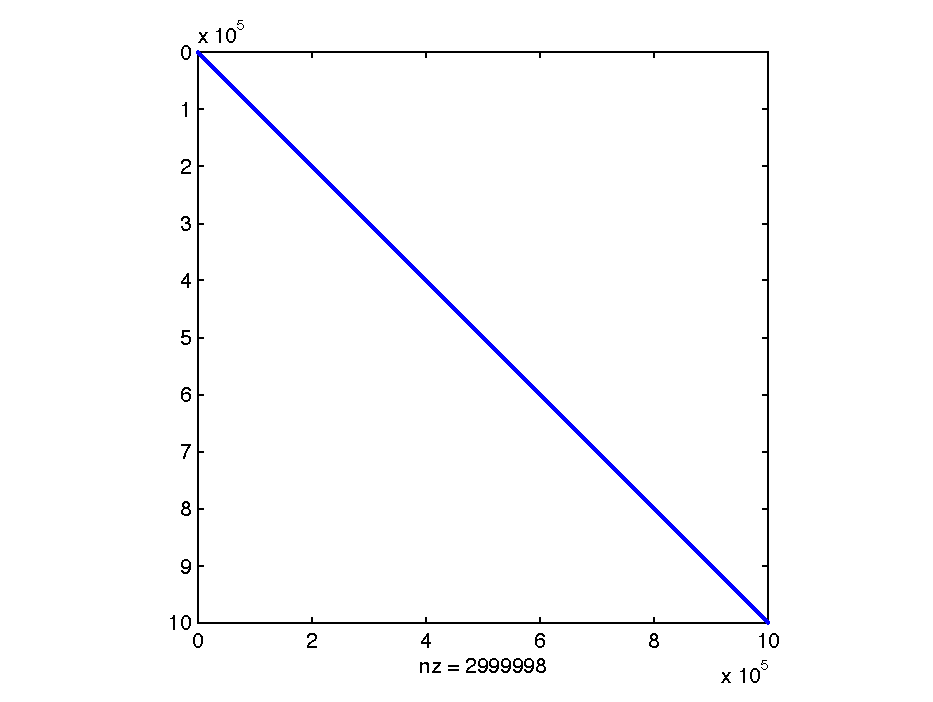
\includegraphics[scale = .5]{./FiguresMAT/spy}
\end{center}
\caption{The output of the \li{spy} command.}
\end{figure}

\section*{Using Sparse Matrices}

Consider the linear system $A x = b$, where $A$ is a
 $100,\!000\times 100,\!000$ tri-diagonal matrix.  To store a full
matrix of that size in your computer, it would normally require 10
billion double-precision floating-point numbers.  Since it takes 8
bytes to store a double, it would take roughly 80GB to store the
full matrix.  For most desktop computers, that fact alone makes the
system numerically prohibitive to solve. The temporal complexity of the problem is even more problematic. Methods for directly solving an arbitrary linear system are usually $O(n^3)$.  As
a result, even if the computer could store an 80GB matrix in RAM, it
would still take several weeks to solve the system.  However, since
we don't have computers with that much available RAM, most of the
matrix would have to be stored on the hard drive, so the computation
would probably take between $6$ months to a year.

The point is that even the next generation of computers will
struggle with solving arbitrary linear systems of this size in a
reasonable period of time.  However, if we take advantage of the
sparse structure of the tri-diagonal matrix, we can solve the linear
system, even with a modest modern computer.  This is because all of
those zeros don't need to be stored and we don't need to do as many
operations to row reduce the tri-diagonal system.

Let's first compute the spatial complexity of the above system when
considered as a sparse matrix.  There are three diagonals that have
roughly $100,\!000$ non-zero entries.  That's $300,\!000$
double-precision floating point numbers, which is about 2.4 MB (Less
storage than your favorite song).  As a result, it will easily
fit into the computer's RAM.  Furthermore, the temporal complexity for solving
a tri-diagonal matrix is $O(n)$. Let's see how long it takes to
solve the system for random data:

\begin{lstlisting}[style=matlab]
>> D = rand(100000,3);
>> b = rand(100000,1);
>> A = spdiags(D,-1:1,100000,100000);
>> tic; A \ b; toc
\end{lstlisting}

\begin{problem}
Write a MATLAB script that returns a full $n\times n$
tri-diagonal matrix with $2$'s along the diagonal and $-1$'s along
the two sub-diagonals above and below the diagonal. Hint: Use the \li{teoplitz} command. Note that this is the second derivative matrix that we discussed at the beginning of this lab.
\end{problem}

\begin{problem}
Repeat the above except have the script return a sparse
matrix. You must build this as a sparse matrix from the beginning. Hint: Use the \li{spdiags} command.
\end{problem}

\begin{problem}
Solve the linear system $A x = b$ where $A$ is the $n\times n$
tri-diagonal matrix from the above two problems and $b$ is randomly
generated.  How high can you go for each method?  Make a table for
several different values of $n$ and the time it took to solve for
each run.  What conclusions can you draw?
\end{problem}

\begin{problem}
Using the sparse matrix above and the command \li{eigs}, calculate the smallest eigenvalue $\lambda$ of the matrix as the matrix's size goes to infinity. What value does $\lambda n^2$ approach (It's the square of an important number)? This is related to operator theory: the second derivative operator has this eigenvalue in certain cases.
\end{problem}

\section*{Other Sparse Commands}

One important command for sparse matrices is the \li{nnz} command, which is related to the number of nonzero entries in a matrix. You can actually pass any matrix into the \li{nnz} function and it returns how many entries are non-zero. When using MATLAB's sparse matrix representation this number is particularly important since it is an indicator of the amount of time and space that is required to operate on the matrix. You should be aware that there is some overhead to using and storing the sparse matrix data structure. Sparsely represented matrices are very beneficial when the number of non-zero entries is relatively small compared to the total number of entries. When the matrix has many non-zero entries, a sparse representation becomes disadvantageous. To see this, create and execute a script with the following code:

\begin{lstlisting}[style=matlab]
A = rand(600); tic; B = A^2; toc
A = sparse(A); tic; B = A^2; toc
\end{lstlisting}
Run the script and note the two different run-times. Notice that it takes about twice as long to perform the operation with the sparse matrix. This is because the sparse matrix data structure is optimized for matrices that are acutally sparse. The matrix $A$ is entirely non-zero. Thus, you incur the overhead of the sparse matrix representation without any benefits since there are no entries you are not required to store or compute. To summarize, only use MATLAB's sparse matrix data structure when your matrices are in fact sparse. Using sparse matrices for mostly full matrices will hurt your performance and memory requirements.

Another important command is the \li{spalloc} command. Sometimes it is necessary to create sparse matrices that do not have a nice banded pattern. To create a general matrix you can operate on, use the \li{spalloc} function. This function takes three arguments: \li{m}, \li{n}, \li{nnzmax}. \li{M} is the number of rows in the matrix, \li{n} is the number of columns, and \li{nnzmax} is the number of nonzero entries you expect the sparse matrix to hold. For example,
\begin{lstlisting}[style=matlab]
A = spalloc(100, 200, 3);
A(1, 34) = 23;
A(23, 32) = 12;
A(99, 109) = 1.23;
\end{lstlisting}
This code snippet creates a $100 \times 200$ sparse matrix with room
for 3 non-zero entries. When the matrix is created all of the entries
are initially assumed to be zero. Notice that we can use the normal
indexing conventions to assign values to these entries. In fact, we
operate on sparse matrices exactly as if they were normal matrices,
except that MATLAB uses special sparse matrix operations to take
advantage of the sparse structure.

The arguments \li{m} and \li{n} in \li{spalloc} are pretty obvious. However,
\li{nnzmax} is a little more subtle. Maybe you don't know exactly how
many nonzero entries you will have; that is OK. When you use {\tt
spalloc} to create a sparse matrix, MATLAB sets aside space for
\li{nnzmax} nonzero entries. When the matrix is created, all of the
entries are assumed to be zero, but the matrix still takes up enough
memory to store \li{nnzmax} entries. If you don't end up using all of
them, the matrix will still operate fast, it will just take up more
space than is needed. What happens if you try to create more
non-zero entries than the \li{nnzmax} value you assigned? This is just
fine as well, except that in this case, MATLAB has to create extra
space for these entries. It is important to note that allocating
space after the matrix is created is time consuming, so you
don't want to do it too often. In general it is probably more
efficient to overestimate the number of entries you will use and
waste a little memory than to do a bunch of allocations because your
NNZMAX value was too small.

For example, type the following script into MATLAB (don't worry if you don't understand all of the syntax, you will very soon):

\begin{lstlisting}[style=matlab]
n = 1e5;
A = spalloc(n,n,n);
B = spalloc(n,n,1);
tic;
for i = 1:n
    A(1,i) = rand(1);
end
toc
tic;
for i = 1:n
    B(1,i) = rand(1);
end
toc
\end{lstlisting}

This script creates two sparse matrices, each $100,\!000 \times 100,\!000$. The difference between the two is that one has pre-allocated $100,\!000$ entries, while the other has only allocated one. We then populate the entries of each matrix the same way, adding a random number one by one. Try running this script. The second method takes significantly longer, and is completely due to pre-allocation.
